\documentclass[twoside]{book}

\usepackage[paperwidth=148mm, paperheight=210mm]{geometry}
\usepackage{fontspec}
%\usepackage[latin1]{inputenc}
\usepackage[nolocalmarks]{polyglossia}
\setdefaultlanguage[variant=french, frenchitemlabels=false]{french}
\usepackage[strict]{changepage}
\usepackage{fancyhdr}
\usepackage{paracol}
\usepackage{tableof}
\usepackage{setspace}
\usepackage{alltt}
\usepackage{titlesec}
\usepackage{xcolor}
\usepackage{xstring}
\usepackage{enumitem}

%%%%%%%%%%%%%%%%%%%%%%%%%%%%%%%%%%%%%%%%%%%%%%%%%%% Mise ne page %%%%%%%%%%%%%%%%%%%%%%%%%%%%%%
% on numérote les nbp par page et non globalement
\usepackage[perpage]{footmisc}

% définition des en-têtes et pieds de page
\pagestyle{empty}
\fancyhead{}
\fancyfoot{}
\renewcommand{\headrulewidth}{0pt}
\setlength{\headheight}{10pt}
\fancyhead[RO]{\small\thepage}
\fancyhead[LE]{\small\thepage}
% la commande titres permet de changer les titres de gauche et de droite.
\newcommand{\titres}[2]{
	\renewcommand{\rightmark}{\textcolor{red}{\sc #2}}
	\renewcommand{\leftmark}{\textcolor{red}{\sc #1}}
}
\titres{}{}

% pas d'indentation
\setlength{\parindent}{0mm}

\geometry{
inner=25mm,
outer=12mm,
top=15mm,
bottom=15mm,
headsep=3mm,
}

%%%%%%%%%%%%%%%%%%%%%%%%%%%%%%%%%%%%%%%%%%%%%%%%% Options gregorio %%%%%%%%%%%%%%%%%%%%%%%%%

\usepackage[forcecompile]{gregoriotex}
%\usepackage{gregoriotex}

%% style général de gregorio :
% lignes rouges, commenter pour du noir
%\gresetlinecolor{gregoriocolor}

% texte <alt> (au-dessus de la portée) en rouge et en petit, avec réglage de sa position verticale
\grechangestyle{abovelinestext}{\color{gregoriocolor}\footnotesize}
\newcommand{\altraise}{-1.4mm}
\grechangedim{abovelinestextraise}{\altraise}{scalable}

% taille des initiales
\newcommand{\initialsize}[1]{
    \grechangestyle{initial}{\fontspec{Zallman Caps}\fontsize{#1}{#1}\selectfont}
}
\newcommand{\defaultinitialsize}{28}
\initialsize{\defaultinitialsize}
% espace avant et après les initiales
\newcommand{\initialspace}[1]{
  \grechangedim{afterinitialshift}{#1}{scalable}
  \grechangedim{beforeinitialshift}{#1}{scalable}
}
\newcommand{\defaultinitialspace}{0cm}
\initialspace{\defaultinitialspace}


% on définit le système qui capture des headers pour générer des annotations
% cette commande sera appelée pour définir des abréviations ou autres substitutions
\newcommand{\resultat}{}
\newcommand{\abbrev}[3]{
  \IfSubStr{#1}{#2}{ \renewcommand{\resultat}{#3} }{}
}
\newcommand{\officepartannotation}[1]{
  \renewcommand{\resultat}{#1}
  \abbrev{#1}{ntro}{ {Intr.} }
  \abbrev{#1}{espo}{Resp.}
  \abbrev{#1}{ll}{All.}
  \abbrev{#1}{act}{Tract.}
  \abbrev{#1}{equen}{Seq.}
  \abbrev{#1}{ffert}{Off.}
  \abbrev{#1}{ommun}{Co.}
  \abbrev{#1}{ntip}{Ant.}
  \abbrev{#1}{ntic}{Cant.}
  \abbrev{#1}{Toni Communes}{}
  \abbrev{#1}{yrial}{}
  \greannotation{\resultat}
}
\newcommand{\modeannotation}[1]{
  \renewcommand{\resultat}{#1}
  \abbrev{#1}{1}{ {\sc i} }
  \abbrev{#1}{2}{ {\sc ii} }
  \abbrev{#1}{3}{ {\sc iii} }
  \abbrev{#1}{4}{ {\sc iv} }
  \abbrev{#1}{5}{ {\sc v} }
  \abbrev{#1}{6}{ {\sc vi} }
  \abbrev{#1}{7}{ {\sc vii} }
  \abbrev{#1}{8}{ {\sc viii} }
  \greannotation{\resultat}
}
\gresetheadercapture{office-part}{officepartannotation}{}
\gresetheadercapture{mode}{modeannotation}{string}

%%%%%%%%%%%%%%%%%%%%%%%%%%%%%%%%%%%%%%%%%%%%%% Graphisme %%%%%%%%%%%%%%%%%%%%%%%%%%%
% on définit l'échelle générale

\newcommand{\echelle}{0.85}

% on centre les titres et on ne les numérote pas
\titleformat{\section}[block]{\Large\filcenter\sc}{}{}{}
\titleformat{\subsection}[block]{\large\filcenter\sc}{}{}{}
\titleformat{\paragraph}[block]{\filcenter\sc}{}{}{}
\setcounter{secnumdepth}{0}
% on diminue l'espace avant les titres
\titlespacing*{\paragraph}{0pt}{1ex}{.6ex}

% commandes versets, repons et croix
\newcommand{\vv}{\textcolor{red}{\fontspec[Scale=\echelle]{Charis SIL}℣.\hspace{3mm}}}
\newcommand{\rr}{\textcolor{red}{\fontspec[Scale=\echelle]{Charis SIL}℟.\hspace{3mm}}}
\newcommand{\cc}{\textcolor{red}{\fontspec[Scale=\echelle]{FreeSerif}\symbol{"2720}~}}
\renewcommand{\aa}{\textcolor{red}{\fontspec[Scale=\echelle]{Charis SIL}\Abar.\hspace{3mm}}}
\gresetspecial{V/}{\textcolor{gregoriocolor}{\fontspec{Charis SIL}℣.~}}
\gresetspecial{R/}{\textcolor{gregoriocolor}{\fontspec{Charis SIL}℟.~}}
\gresetspecial{A/}{\textcolor{gregoriocolor}{\fontspec{Charis SIL}\Abar.~}}
\gresetspecial{+}{{\fontspec{FreeSerif}†~}}
\gresetspecial{*}{\gresixstar}
\gresetspecial{cross}{\textcolor{gregoriocolor}{\fontspec{FreeSerif}\symbol{"2720}}}
\gresetspecial{labiacross}{\textcolor{gregoriocolor}{+}}

% commandes diverses
\newcommand{\antiphona}{\textcolor{red}{\noindent Antiphona.\hspace{4mm}}}
\newcommand{\antienne}{\textcolor{red}{\noindent Antienne.\hspace{4mm}}}
\newcommand{\rubrique}[1]{\textcolor{red}{\emph{#1}}}
\newcommand{\saut}{\hspace{1cm}}
\newcommand{\minisaut}{\hspace{4mm}}
\newcommand{\sautRV}{\\ \null \hspace{5.95mm}}
\newcommand{\petitvspace}{\vspace{2mm}}
\newcommand{\microvspace}{\vspace{0.8mm}}
% pour affichier 1 en rouge et un peu d'espace
\newcommand{\un}{{\color{gregoriocolor} 1~~~}}

% abréviations
\newcommand{\tpalleluia}{\rubrique{(T.P.} \mbox{Allelúia.\rubrique{)}}}
\newcommand{\tpalleluiafr}{\rubrique{(T.P.} \mbox{Alléluia.\rubrique{)}}}

\newcommand{\tqomittitur}{{\small \rubrique{(In Tempore Quadragesimæ ommittitur} Allelúia.\rubrique{)}}}
\newcommand{\careme}{{\small \rubrique{(Pendant le Carême on omet l'}Alléluia.\rubrique{)}}}

% environnement hymne : alltt + normalfont + marges custom
\newenvironment{hymne}
  {
  \begin{adjustwidth}{1.6cm}{1mm}
  \begin{alltt}\normalfont
  }
  {
  \end{alltt}
  \end{adjustwidth}
  }
  
% la commande \u permet de souligner les inflexions
\let\u\underline

% on définit la police par défaut
\setmainfont[Ligatures=TeX, Scale=\echelle]{Charis SIL}
%renderer=ICU a l'air de ne plus marcher...
%\setmainfont[Renderer=ICU, Ligatures=TeX, Scale=\echelle]{Charis SIL}
\setstretch{0.9}

% paramétrage de paracol en mode 2 colonnes par page : taille des colonnes, séparateur
\columnratio{0.5}
\setlength{\columnsep}{1.5em}
\setlength{\columnseprule}{0.3pt}

\begin{document}

% ceci est pour conserver une numérotation ordinaire malgré paracol
\twosided[pb]

\begin{titlepage}
\centering\null

\vspace{1cm}

{\scshape\LARGE In Octava Nativitatis}

\vspace{2cm}

{\scshape\Large Ad Matutinum}

\vspace{5cm}

{\scshape\LARGE Octave de Noël}

\vspace{2cm}

{\scshape\Large À Matines}


\end{titlepage}

% tolérance infinie sur les sauts de lignes pour les colonnes étroites
\sloppy
\gresetinitiallines{0}
\gregorioscore{partitions/ORIa}
\gresetinitiallines{1}
\emph{\vv Seigneur, ouvre mes lèvres. \minisaut \rr Et ma bouche annoncera ta louange. \\
\vv Dieu, viens à mon aide. \minisaut \rr Seigneur, viens vite à notre secours. \\
\vv Gloire au Père, au Fils, et au Saint-Esprit. \minisaut \rr Comme il était au commencement, maintenant et toujours, et dans les siècles des siècles. Amen. Alléluia.}

\section{Invitatoire}

\emph{\aa Le Christ nous est né, venez, adorons.}

\gregorioscore{partitions/in--christus_natus_est_nobis--.gabc}

\emph{Venez, chantons avec allégresse au Seigneur, faisons monter l'expression d'une joie vers Dieu, notre salut.
Hâtons-nous de nous présenter devant lui avec des louanges et, dans des psaumes célébrons sa gloire.\\
Parce que le Seigneur est le grand Dieu; le grand Roi au dessus de tous les dieux; parce que le Seigneur ne repoussera pas son peuple; parce que dans sa main sont tous les confins de la terre et que son regard domine les cimes des montagnes.\\
Parce qu'à lui est la mer, et que c'est lui-même qui l'a faite, et que ses mains ont formé le continent. Venez, adorons, prosternons-nous devant Dieu, et pleurons devant le Seigneur qui nous a faits, parce que lui-même est le Seigneur notre Dieu, et que nous sommes son peuple et les brebis de son pâturage.\\
Aujourd'hui, si vous entendez sa voix, n'endurcissez pas vos cœurs, comme il arriva à vos pères dans l'exaspération au jour de la tentation dans le désert, alors qu'ils me tentèrent, m'éprouvèrent et virent mes œuvres.\\
Pendant quarante ans, j'ai été proche de cette génération et j'ai dit: Toujours ils errent de cœur; et eux, ils n'ont point connu mes voies: et je leur ai juré dans ma colère, s'ils entreront dans mon repos.}

\newpage
\section{Hymne}
%\gregorioscore{partitions/hy--jesu_redemptor_omnium_(t._nativitatis)--solesmes_1961.gabc}
\gregorioscore{partitions/hy--christe_redemptor_omnium_ex_patre--solesmes_1934.gabc}

~

\begin{paracol}{2}
\begin{alltt}\normalfont        O Christ, ô rédempteur de tous
        issu du Père Fils unique
        toi seul, avant le principe
        es né inexprimablement.

        Splendeur du Père et son éclat
        espoir à jamais de tout homme
        écoute le flot des pières
        de cux qui te servent partout.
        
        Auteur du salut, souviens-toi :
        naguère tu as pris la forme
        de notre corps, en ta naissance
        d'une femme au sein virginal.\end{alltt}
\switchcolumn
\begin{alltt}\normalfont    Ce jour présent en est témoin,
    que le cycle de l'an ramène :
    seul, quittant le séjour du Père,
    tu vins sauver le monde entier.

    Le ciel et la terre et la mer
    et tous les êtres qu'ils contiennent
    louent, dans la joie de leur cantique,
    ce jour de ton avènement.
    
    Et nous les hommes, nous aussi,
    que ton sang précieux rachète,
    fêtons le jour de ta naissance,
    et entonnons le chant nouveau.\end{alltt}
\end{paracol}

\section{Premier nocturne}

\subsection{Psaume 2}

\gregorioscore{partitions/an1--dominus_dixit_ad_me--nocturnale_2002.gabc}
\gresetinitiallines{0}
\gregorioscore{partitions/ps1_2.gabc}
\gresetinitiallines{1}
\aa \emph{Le Seigneur m'a dit: tu es mon Fils, aujourd'hui, je t'ai engendré.}

\un \emph{Pourquoi ce tumulte des nations, ce vain murmure des peuples?}
\begin{paracol}{2}
\begin{enumerate}[wide, itemsep=0mm, labelwidth=!, labelindent=0pt, label=\color{gregoriocolor}\theenumi]
\setcounter{enumi}{1}
\item Astitérunt reges terræ, et príncipes convenérunt in \textbf{u}num~* advérsus Dóminum, et advérsus \textit{Chris}\textit{tum} \textbf{e}jus.
\item Dirumpámus víncula e\textbf{ó}rum:~* et projiciámus a nobis ju\textit{gum} \textit{ip}\textbf{só}rum.
\item Qui hábitat in cælis, irridébit \textbf{e}os:~* et Dóminus subsan\textit{ná}\textit{bit} \textbf{e}os.
\item Tunc loquétur ad eos in ira \textbf{su}a,~* et in furóre suo contur\textit{bá}\textit{bit} \textbf{e}os.
\item Ego autem constitútus sum Rex ab eo super Sion montem sanctum \textbf{e}jus,~* prǽdicans præ\textit{cép}\textit{tum} \textbf{e}jus.
\item Dóminus dixit \textbf{ad} me:~* Fílius meus es tu, ego hódie \textit{gé}\textit{nu}\textbf{i} te.
\item Póstula a me, et dabo tibi Gentes hereditátem \textbf{tu}am,~* et possessiónem tuam tér\textit{mi}\textit{nos} \textbf{ter}ræ.
\item Reges eos in virga \textbf{fér}rea,~* et tamquam vas fíguli con\textit{frín}\textit{ges} \textbf{e}os.
\item Et nunc, reges, intel\textbf{lí}gite:~* erudímini, qui judi\textit{cá}\textit{tis} \textbf{ter}ram.
\item Servíte Dómino in ti\textbf{mó}re:~* et exsultáte ei \textit{cum} \textit{tre}\textbf{mó}re.
\item Apprehéndite disciplínam, nequándo irascátur \textbf{Dó}minus,~* et pereátis de \textit{vi}\textit{a} \textbf{jus}ta.
\item Cum exárserit in brevi ira \textbf{e}jus:~* beáti omnes qui confí\textit{dunt} \textit{in} \textbf{e}o.
\item Glória Patri, et \textbf{Fí}lio,~* et Spirí\textit{tu}\textit{i} \textbf{Sanc}to.
\item Sicut erat in princípio, et nunc, et \textbf{sem}per,~* et in sǽcula sæcu\textit{ló}\textit{rum}. \textbf{A}men.
\end{enumerate}
\switchcolumn
\begin{enumerate}[wide, itemsep=0mm, labelwidth=!, labelindent=0pt, before=\itshape, label=\color{gregoriocolor}\theenumi]
\setcounter{enumi}{1}
\item Les rois de la terre se dressent, les grands se liguent entre eux contre le Seigneur et son messie:
\item «Faisons sauter nos chaînes, rejetons ces entraves !»
\item Celui qui règne dans les cieux s'en amuse, le Seigneur les tourne en dérision;
\item puis il leur parle avec fureur, et sa colère les épouvante:
\item «Moi, j'ai sacré mon roi sur Sion, ma sainte montagne.»
\item Je proclame le décret du Seigneur! Il m'a dit: «Tu es mon fils; moi, aujourd'hui, je t'ai engendré.
\item Demande, et je te donne en héritage les nations, pour domaine la terre tout entière.
\item Tu les détruiras de ton sceptre de fer, tu les briseras comme un vase de potier.»
\item Maintenant, rois, comprenez, reprenez-vous, juges de la terre.
\item Servez le Seigneur avec crainte, rendez-lui votre hommage en tremblant.
\item Qu'il s'irrite et vous êtes perdus: soudain sa colère éclatera. 
\item Heureux qui trouve en lui son refuge!
\item Gloire au Père, au Fils, et au Saint-Esprit.
\item Comme il était au commencement, maintenant et toujours, dans les siècles des siècles. Amen.
\end{enumerate}
\end{paracol}

\subsection{Psaume 18}

\gregorioscore{partitions/an2--in_sole_posuit_tabernaculum--nocturnale_2002.gabc}
\gresetinitiallines{0}
\gregorioscore{partitions/ps2_18.gabc}
\gresetinitiallines{1}
\aa \emph{C'est dans le soleil qu'il a placé son tabernacle; et lui-même, comme l'époux, il sort de la chambre nuptiale.}

\un \emph{Les cieux proclament la gloire de Dieu, le firmament raconte l'ouvrage de ses mains.}
\begin{paracol}{2}
\begin{enumerate}[wide, itemsep=0mm, labelwidth=!, labelindent=0pt, label=\color{gregoriocolor}\theenumi]
\setcounter{enumi}{1}
\item Dies diéi erúctat \textbf{ver}bum,~* et nox nocti índi\textbf{cat} sci\textbf{én}tiam.
\item Non sunt loquélæ, neque ser\textbf{mó}nes,~* quorum non audiántur \textbf{vo}ces e\textbf{ó}rum.
\item In omnem terram exívit sonus e\textbf{ó}rum:~* et in fines orbis terræ \textbf{ver}ba e\textbf{ó}rum.
\item In sole pósuit tabernáculum \textbf{su}um:~* et ipse tamquam sponsus procédens de \textbf{thá}lamo \textbf{su}o.
\item Exsultávit ut gigas ad curréndam \textbf{vi}am,~* a summo cælo e\textbf{grés}sio \textbf{e}jus.
\item Et occúrsus ejus usque ad summum \textbf{e}jus:~* nec est qui se abscóndat a ca\textbf{ló}re \textbf{e}jus.
\item Lex Dómini immaculáta, convértens \textbf{á}nimas:~* testimónium Dómini fidéle, sapiéntiam \textbf{præ}stans \textbf{pár}vulis.
\item Justítiæ Dómini rectæ, lætificántes \textbf{cor}da:~* præcéptum Dómini lúcidum il\textbf{lú}minans \textbf{ó}culos.
\item Timor Dómini sanctus, pérmanens in sǽculum \textbf{sǽ}culi:~* judícia Dómini vera, justificáta in \textbf{se}met\textbf{íp}sa.
\item Desiderabília super aurum et lápidem pretiósum \textbf{mul}tum:~* et dulcióra super \textbf{mel} et \textbf{fa}vum.
\item Etenim servus tuus custódit \textbf{e}a,~* in custodiéndis illis retri\textbf{bú}tio \textbf{mul}ta.
\item Delícta quis intélligit?~† ab occúltis meis \textbf{mun}da me:~* et ab aliénis parce \textbf{ser}vo \textbf{tu}o.
\item Si mei non fúerint domináti, tunc immaculátus \textbf{e}ro:~* et emundábor a de\textbf{líc}to \textbf{má}ximo.
\item Et erunt ut compláceant elóquia oris \textbf{me}i:~* et meditátio cordis mei in conspéctu \textbf{tu}o \textbf{sem}per.
\item Dómine, adjútor \textbf{me}us,~* et red\textbf{émp}tor \textbf{me}us.
\item Glória Patri, et \textbf{Fí}lio,~* et Spi\textbf{rí}tui \textbf{Sanc}to.
\item Sicut erat in princípio, et nunc, et \textbf{sem}per,~* et in sǽcula sæcu\textbf{ló}rum. \textbf{A}men.
\end{enumerate}
\switchcolumn
\begin{enumerate}[wide, itemsep=0mm, labelwidth=!, labelindent=0pt, before=\itshape, label=\color{gregoriocolor}\theenumi]
\setcounter{enumi}{1}
\item Le jour au jour en livre le récit et la nuit à la nuit en donne connaissance.
\item Pas de paroles dans ce récit, pas de voix qui s'entende;
\item mais sur toute la terre en paraît le message et la nouvelle, aux limites du monde. 
\item Là, se trouve la demeure du soleil: tel un époux, il paraît hors de sa tente,
\item il s'élance en conquérant joyeux. Il paraît où commence le ciel,
\item il s'en va jusqu'où le ciel s'achève: rien n'échappe à son ardeur.
\item La loi du Seigneur est parfaite, qui redonne vie; la charte du Seigneur est sûre, qui rend sages les simples.
\item Les préceptes du Seigneur sont droits, ils réjouissent le cœur; le commandement du Seigneur est limpide, il clarifie le regard.
\item La crainte qu'il inspire est pure, elle est là pour toujours; les décisions du Seigneur sont justes et vraiment équitables:
\item plus désirables que l'or, qu'une masse d'or fin, plus savoureuses que le miel qui coule des rayons.
\item Aussi ton serviteur en est illuminé; à les garder, il trouve son profit.
\item Qui peut discerner ses erreurs? Purifie-moi de celles qui m'échappent.
\item Préserve aussi ton serviteur de l'orgueil: qu'il n'ait sur moi aucune emprise. Alors je serai sans reproche, pur d'un grand péché.
\item Accueille les paroles de ma bouche, le murmure de mon cœur; qu'ils parviennent devant toi, 
\item Seigneur, mon rocher, mon défenseur!
\item Gloire au Père, au Fils, et au Saint-Esprit.
\item Comme il était au commencement, maintenant et toujours, dans les siècles des siècles. Amen.
\end{enumerate}
\end{paracol}

\subsection{Psaume 23}

\gregorioscore{partitions/an3--elevamini--nocturnale_2002.gabc}
\gresetinitiallines{0}
\gregorioscore{partitions/ps3_23.gabc}
\gresetinitiallines{1}
\aa \emph{Levez-vous, portes éternelles, qu'il entre, le Roi de gloire.}

\un \emph{Au Seigneur, le monde et sa richesse, la terre et tous ses habitants!}
\begin{paracol}{2}
\begin{enumerate}[wide, itemsep=0mm, labelwidth=!, labelindent=0pt, label=\color{gregoriocolor}\theenumi]
\setcounter{enumi}{1}
\item Quia ipse super mária fundávit \textbf{e}um:~* et super flúmina præpa\textbf{rá}vit \textbf{e}um.
\item Quis ascéndet in montem \textbf{Dó}mini?~* aut quis stabit in loco \textbf{sanc}to \textbf{e}jus?
\item Innocens mánibus et mundo corde,~† qui non accépit in vano ánimam \textbf{su}am,~* nec jurávit in dolo \textbf{pró}ximo \textbf{su}o.
\item Hic accípiet benedictiónem a \textbf{Dó}mino:~* et misericórdiam a Deo, salu\textbf{tá}ri \textbf{su}o.
\item Hæc est generátio quæréntium \textbf{e}um,~* quæréntium fáciem \textbf{De}i \textbf{Ja}cob.
\item Attóllite portas, príncipes, vestras,~† et elevámini, portæ æter\textbf{ná}les:~* et intro\textbf{í}bit Rex \textbf{gló}riæ.
\item Quis est iste Rex glóriæ?~† Dóminus fortis et \textbf{pot}ens:~* Dóminus \textbf{pot}ens in \textbf{prǽ}lio.
\item Attóllite portas, príncipes, vestras,~† et elevámini, portæ æter\textbf{ná}les:~* et intro\textbf{í}bit Rex \textbf{gló}riæ.
\item Quis est iste Rex \textbf{gló}riæ?~* Dóminus virtútum ipse \textbf{est} Rex \textbf{gló}riæ.
\item Glória Patri, et \textbf{Fí}lio,~* et Spi\textbf{rí}tui \textbf{Sanc}to.
\item Sicut erat in princípio, et nunc, et \textbf{sem}per,~* et in sǽcula sæcu\textbf{ló}rum. \textbf{A}men.
\end{enumerate}
\switchcolumn
\begin{enumerate}[wide, itemsep=0mm, labelwidth=!, labelindent=0pt, before=\itshape, label=\color{gregoriocolor}\theenumi]
\setcounter{enumi}{1}
\item C'est lui qui l'a fondée sur les mers et la garde inébranlable sur les flots.
\item Qui peut gravir la montagne du Seigneur et se tenir dans le lieu saint?
\item L'homme au cœur pur, aux mains innocentes, qui ne livre pas son âme aux idoles, et ne dit pas de faux serments.
\item Il obtient, du Seigneur, la bénédiction, et de Dieu son Sauveur, la justice.
\item Voici le peuple de ceux qui le cherchent! Voici Jacob qui recherche ta face!
\item Portes, levez vos frontons, élevez-vous, portes éternelles: qu'il entre, le roi de gloire!
\item Qui est ce roi de gloire? C'est le Seigneur, le fort, le vaillant, le Seigneur, le vaillant des combats.
\item Portes, levez vos frontons, levez-les, portes éternelles: qu'il entre, le roi de gloire!
\item Qui donc est ce roi de gloire? C'est le Seigneur, Dieu de l'univers; c'est lui, le roi de gloire.
\item Gloire au Père, au Fils, et au Saint-Esprit.
\item Comme il était au commencement, maintenant et toujours, dans les siècles des siècles. Amen.
\end{enumerate}
\end{paracol}

\subsection{Versicule}
\begin{paracol}{2}
\vv Tamquam sponsus. \\
\rr Dóminus procédens de thálamo suo. \\
\vv Pater noster... \rubrique{(secrètement)} Et ne nos indúcas in tentatiónem. \\
\rr Sed líbera nos a malo. \\
\vv Exáudi, Dómine Iesu Christe, preces servórum tuórum, et miserére nobis: Qui cum Patre et Spíritu Sancto vivis et regnas in sǽcula sæculórum. \rr Amen.
\switchcolumn
\vv Comme l'époux. \\
\rr Le Seigneur sort de sa chambre. \\
\vv Notre Père... Et ne nous laissez pas succomber à la tentation. \\
\rr Mais délivrez-nous du mal. \\
\vv Exaucez, Seigneur Jésus-Christ, les prières de vos serviteurs, et ayez pitié de nous, vous qui vivez et régnez avec le Père et le Saint-Esprit, dans les siècles des siècles. \rr Amen.
\end{paracol}

\subsection{Première leçon}

\begin{paracol}{2}
\vv Jube, domne, benedícere. \\
\vv Benedictióne perpétua benedícat nos Pater ætérnus.\\
\rr Amen.\\
\rubrique{Si le célébrant n'est pas au moins diacre, le lecteur dit} Dómine \rubrique{au lieu de} domne\rubrique{.}
\switchcolumn
\vv Veuillez, Seigneur, bénir. \\
\vv Que le Père éternel nous bénisse d'une bénédiction perpétuelle. \\
\rr Amen.
\end{paracol}

\paragraph{Lecture de la lettre de Saint Paul, Apôtre, aux Romains} \rubrique{Rom 4: 1-8}

Que dirons-nous alors d’Abraham, notre ancêtre selon la chair? Qu’a-t-il obtenu?
Si Abraham était devenu un homme juste par la pratique des œuvres, il aurait pu en tirer fierté, mais pas devant Dieu.
Or, que dit l’Écriture? Abraham eut foi en Dieu, et il lui fut accordé d’être juste.
Si quelqu’un accomplit un travail, son salaire ne lui est pas accordé comme un don gratuit, mais comme un dû.
Au contraire, si quelqu’un, sans rien accomplir, a foi en Celui qui rend juste l’homme impie, il lui est accordé d’être juste par sa foi.
C’est ainsi que le psaume de David proclame heureux l’homme à qui Dieu accorde d’être juste, indépendamment de la pratique des œuvres:
Heureux ceux dont les offenses ont été remises, et les péchés, effacés.
Heureux l’homme dont le péché n’est pas compté par le Seigneur.

\begin{paracol}{2}
\vv Tu autem, Dómine, miserére nobis. \\
\rr Deo grátias.
\switchcolumn
\vv Et vous Seigneur, ayez pitié de nous. \\
\rr Rendons grâces à Dieu.
\end{paracol}

\gregorioscore{partitions/re1--ecce_agnus_dei_(resp.)--gregofacsimil.gabc}

\emph{\rr Voici l'Agneau de Dieu, celui qui porte le péché du monde. C'est de lui que je vous ai dit: celui qui vient après moi était avant moi, et je ne suis pas digne de délier la courroie de sa sandale.
\vv Celui qui est de la terre, parle de la terre ; celui qui vient du ciel, est au-dessus de tous.}

\subsection{Deuxième leçon}

\begin{paracol}{2}
\vv Jube, domne, benedícere. \\
\vv Unigénitus Dei Fílius nos benedícere et adjuváre dignétur.\\
\rr Amen.
\switchcolumn
\vv Veuillez, Seigneur, bénir. \\
\vv Que le Fils unique de Dieu daigne nous bénir et nous secourir.\\
\rr Amen.
\end{paracol}

\rubrique{Rom 4: 9-12}

Cette béatitude-là concerne-t-elle seulement ceux qui ont la circoncision, ou bien aussi ceux qui ne l’ont pas? Nous disons, en effet: «C’est pour sa foi qu’il a été accordé à Abraham d’être juste.»
Et quand cela lui fut-il accordé? Après la circoncision? ou avant? Non pas après, mais avant.
Et il reçut le signe de la circoncision comme la marque de la justice obtenue par la foi avant d’être circoncis. De cette façon, il est le père de tous ceux qui croient sans avoir la circoncision, pour qu’à eux aussi, il soit accordé d’être justes;
et il est également le père des circoncis, ceux qui non seulement ont la circoncision, mais qui marchent aussi sur les traces de la foi de notre père Abraham avant sa circoncision.

\begin{paracol}{2}
\vv Tu autem, Dómine, miserére nobis. \\
\rr Deo grátias.
\switchcolumn
\vv Et vous Seigneur, ayez pitié de nous. \\
\rr Rendons grâces à Dieu.
\end{paracol}

\gregorioscore{partitions/re2--dies_sanctificatus_illuxit_(resp.)--gregofacsimil.gabc}

\emph{\rr Un jour saint nous illumine: venez, peuples, et adorez le Seigneur, car aujourd'hui une grande lumière est descendue sur la terre. \\
\vv Voici le jour qu’a fait le Seigneur ; réjouissons-nous et tressaillons d’allégresse en ce jour.
}

~

\subsection{Troisième leçon}

~

\begin{paracol}{2}
\vv Jube, domne, benedícere. \\
\vv Spíritus Sancti grátia illúminet sensus et corda nostra.\\
\rr Amen.
\switchcolumn
\vv Veuillez, Seigneur, bénir. \\
\vv Que la grâce du Saint-Esprit illumine nos esprits et nos cœurs.\\
\rr Amen.
\end{paracol}

\rubrique{Rom 4: 13-17}

Car ce n’est pas en vertu de la Loi que la promesse de recevoir le monde en héritage a été faite à Abraham et à sa descendance, mais en vertu de la justice obtenue par la foi.
En effet, si l’on devient héritier par la Loi, alors la foi est sans contenu, et la promesse, abolie.
Car la Loi aboutit à la colère de Dieu, mais là où il n’y a pas de Loi, il n’y a pas non plus de transgression.
Voilà pourquoi on devient héritier par la foi: c’est une grâce, et la promesse demeure ferme pour tous les descendants d’Abraham, non pour ceux qui se rattachent à la Loi seulement, mais pour ceux qui se rattachent aussi à la foi d’Abraham, lui qui est notre père à tous.
C’est bien ce qui est écrit: J’ai fait de toi le père d’un grand nombre de nations. Il est notre père devant Dieu en qui il a cru, Dieu qui donne la vie aux morts et qui appelle à l’existence ce qui n’existe pas.

\begin{paracol}{2}
\vv Tu autem, Dómine, miserére nobis. \\
\rr Deo grátias.
\switchcolumn
\vv Et vous Seigneur, ayez pitié de nous. \\
\rr Rendons grâces à Dieu.
\end{paracol}

\gregorioscore{partitions/re3--benedictus_qui_venit_(resp.)--gregofacsimil.gabc}

\emph{\rr Béni soit celui qui vient au nom du Seigneur: le Seigneur notre Dieu nous illumine, alléluia, alléluia.
\vv Voici le jour qu’a fait le Seigneur ; réjouissons-nous et tressaillons d’allégresse en ce jour.}

\section{Deuxième nocturne}

\subsection{Psaume 44}

\gregorioscore{partitions/an4--speciosus_forma--sandhofe.gabc}
\gresetinitiallines{0}
\gregorioscore{partitions/ps4_44.gabc}
\gresetinitiallines{1}
\aa \emph{Tu es beau, comme aucun des enfants des hommes, la grâce est répandue sur tes lèvres.}

\un \emph{D'heureuses paroles jaillissent de mon cœur quand je dis mes poèmes pour le roi.}
\begin{paracol}{2}

\begin{enumerate}[wide, itemsep=0mm, labelwidth=!, labelindent=0pt, label=\color{gregoriocolor}\theenumi]
\setcounter{enumi}{1}
\item Lingua mea \textbf{cá}lamus \textbf{scri}bæ:~* velóci\textit{ter} \textit{scri}\textbf{bén}tis.
\item Speciósus forma præ fíliis hóminum,~† diffúsa est grátia in \textbf{lá}biis \textbf{tu}is:~* proptérea benedíxit te Deus \textit{in} \textit{æ}\textbf{tér}num.
\item Accíngere gládio tuo super \textbf{fe}mur \textbf{tu}um,~* \textit{pot}\textit{en}\textbf{tís}sime.
\item Spécie tua et pulchri\textbf{tú}dine \textbf{tu}a:~* inténde, próspere procé\textit{de}, \textit{et} \textbf{re}gna.
\item Propter veritátem, et mansuetúdinem, \textbf{et} jus\textbf{tí}tiam:~* et dedúcet te mirabíliter déx\textit{te}\textit{ra} \textbf{tu}a.
\item Sagíttæ tuæ acútæ, pópuli \textbf{sub} te \textbf{ca}dent:~* in corda inimi\textit{có}\textit{rum} \textbf{Re}gis.
\item Sedes tua, Deus, in \textbf{sǽ}culum \textbf{sǽ}culi:~* virga directiónis virga \textit{re}\textit{gni} \textbf{tu}i.
\item Dilexísti justítiam, et odísti in\textbf{i}qui\textbf{tá}tem:~* proptérea unxit te, Deus, Deus tuus, óleo lætítiæ præ consór\textit{ti}\textit{bus} \textbf{tu}is.
\item Myrrha, et gutta, et cásia a vestiméntis tuis, a dómi\textbf{bus} e\textbf{búr}neis:~* ex quibus delectavérunt te fíliæ regum in ho\textit{nó}\textit{re} \textbf{tu}o.
\item Astitit regína a dextris tuis in vestítu \textbf{de}au\textbf{rá}to:~* circúmdata va\textit{ri}\textit{e}\textbf{tá}te.
\item Audi, fília, et vide, et inclína \textbf{au}rem \textbf{tu}am:~* et oblivíscere pópulum tuum, et domum \textit{pa}\textit{tris} \textbf{tu}i.
\item Et concupíscet Rex de\textbf{có}rem \textbf{tu}um:~* quóniam ipse est Dóminus Deus tuus, et ado\textit{rá}\textit{bunt} \textbf{e}um.
\item Et fíliæ Tyri \textbf{in} mu\textbf{né}ribus~* vultum tuum deprecabúntur: omnes dí\textit{vi}\textit{tes} \textbf{ple}bis.
\item Omnis glória ejus fíliæ \textbf{Re}gis ab \textbf{in}tus,~* in fímbriis áureis circumamícta va\textit{ri}\textit{e}\textbf{tá}tibus.
\item Adducéntur Regi vírgi\textbf{nes} post \textbf{e}am:~* próximæ ejus affe\textit{rén}\textit{tur} \textbf{ti}bi.
\item Afferéntur in lætítia et exsul\textbf{ta}ti\textbf{ó}ne:~* adducéntur in \textit{tem}\textit{plum} \textbf{Re}gis.
\item Pro pátribus tuis nati sunt \textbf{ti}bi \textbf{fí}lii:~* constítues eos príncipes super \textit{om}\textit{nem} \textbf{ter}ram.
\item Mémores erunt \textbf{nó}minis \textbf{tu}i:~* in omni generatióne et gene\textit{ra}\textit{ti}\textbf{ó}nem.
\item Proptérea pópuli confitebúntur tibi \textbf{in} æ\textbf{tér}num:~* et in sǽ\textit{cu}\textit{lum} \textbf{sǽ}culi.
\item Glória \textbf{Pa}tri, et \textbf{Fí}lio,~* et Spirí\textit{tu}\textit{i} \textbf{Sanc}to.
\item Sicut erat in princípio, et \textbf{nunc}, et \textbf{sem}per,~* et in sǽcula sæcu\textit{ló}\textit{rum}. \textbf{A}men.
\end{enumerate}

\switchcolumn
\begin{enumerate}[wide, itemsep=0mm, labelwidth=!, labelindent=0pt, before=\itshape, label=\color{gregoriocolor}\theenumi]
\setcounter{enumi}{1}
\item D'une langue aussi vive que la plume du scribe!
\item Tu es beau, comme aucun des enfants de l'homme, la grâce est répandue sur tes lèvres: oui, Dieu te bénit pour toujours.
\item Guerrier valeureux, porte l'épée de noblesse et d'honneur!
\item Ton honneur, c'est de courir au combat pour la justice, la clémence et la vérité.
\item Ta main jettera la stupeur, les flèches qui déchirent; 
\item sous tes coups, les peuples s'abattront, les ennemis du roi, frappés en plein cœur.
\item Ton trône est divin, un trône éternel; ton sceptre royal est sceptre de droiture:
\item tu aimes la justice, tu réprouves le mal. Oui, Dieu, ton Dieu t'a consacré d'une onction de joie, comme aucun de tes semblables;
\item la myrrhe et l'aloès parfument ton vêtement. Des palais d'ivoire, la musique t'enchante.
\item Parmi tes bien-aimées sont des filles de roi; à ta droite, la préférée, sous les ors d'Ophir.
\item Écoute, ma fille, regarde et tends l'oreille; oublie ton peuple et la maison de ton père:
\item le roi sera séduit par ta beauté. Il est ton Seigneur: prosterne-toi devant lui.
\item Alors, fille de Tyr, les plus riches du peuple, chargés de présents, quêteront ton sourire.
\item Fille de roi, elle est là, dans sa gloire, vêtue d'étoffes d'or;
\item on la conduit, toute parée, vers le roi. Des jeunes filles, ses compagnes, lui font cortège;
\item on les conduit parmi les chants de fête: elles entrent au palais du roi.
\item À la place de tes pères se lèveront tes fils; sur toute la terre tu feras d'eux des princes.
\item Je ferai vivre ton nom pour les âges des âges: 
\item que les peuples te rendent grâce, toujours, à jamais!
\item Gloire au Père, au Fils, et au Saint-Esprit.
\item Comme il était au commencement, maintenant et toujours, dans les siècles des siècles. Amen.
\end{enumerate}

\end{paracol}

\subsection{Psaume 86}

\gregorioscore{partitions/an5--homo_natus_est--nocturnale_2002.gabc}
\gresetinitiallines{0}
\gregorioscore{partitions/ps5_86.gabc}
\gresetinitiallines{1}
\aa \emph{L'homme est né d'elle, c'est sur elle que le Très-Haut l'a fondé.}

\un \emph{Elle est fondée sur les montagnes saintes. Le Seigneur aime les portes de Sion plus que toutes les demeures de Jacob.}
\begin{paracol}{2}
\begin{enumerate}[wide, itemsep=0mm, labelwidth=!, labelindent=0pt, label=\color{gregoriocolor}\theenumi]
\setcounter{enumi}{1}
\item Gloriósa \textbf{dic}ta sunt \textbf{de} te,~* \textbf{cí}vitas \textbf{De}i.
\item Memor ero Rahab, et \textbf{Ba}by\textbf{ló}nis~* sci\textbf{én}ti\textbf{um} me.
\item Ecce alienígenæ, et Tyrus, et pópu\textbf{lus} Æ\textbf{thí}opum,~* hi fu\textbf{é}runt \textbf{il}lic.
\item Numquid Sion dicet:~† Homo, et homo natus \textbf{est} in \textbf{e}a:~* et ipse fundávit \textbf{e}am Al\textbf{tís}simus?
\item Dóminus narrábit in scriptúris popu\textbf{ló}rum, et \textbf{prín}cipum:~* horum, qui fu\textbf{é}runt in \textbf{e}a.
\item Sicut læ\textbf{tán}tium \textbf{óm}nium:~* habitáti\textbf{o} est \textbf{in} te.
\item Glória \textbf{Pa}tri, et \textbf{Fí}lio,~* et Spi\textbf{rí}tui \textbf{Sanc}to.
\item Sicut erat in princípio, et \textbf{nunc}, et \textbf{sem}per,~* et in sǽcula sæcu\textbf{ló}rum. \textbf{A}men.
\end{enumerate}
\switchcolumn
\begin{enumerate}[wide, itemsep=0mm, labelwidth=!, labelindent=0pt, before=\itshape, label=\color{gregoriocolor}\theenumi]
\setcounter{enumi}{1}
\item Pour ta gloire on parle de toi, ville de Dieu!
\item «Je cite l'Égypte et Babylone entre celles qui me connaissent.» 
\item Voyez Tyr, la Philistie, l'Éthiopie: chacune est née là-bas.
\item Mais on appelle Sion: «Ma mère!» car en elle, tout homme est né. C'est lui, le Très-Haut, qui la maintient.
\item Au registre des peuples, le Seigneur écrit: «Chacun est né là-bas.»
\item Tous ensemble ils dansent, et ils chantent: «En toi, toutes nos sources!
\item Gloire au Père, au Fils, et au Saint-Esprit.
\item Comme il était au commencement, maintenant et toujours, dans les siècles des siècles. Amen.
\end{enumerate}
\end{paracol}

\subsection{Psaume 95}

\gregorioscore{partitions/an6--exsultabunt_omnia_ligna--nocturnale_2002.gabc}
\gresetinitiallines{0}
\gregorioscore{partitions/ps6_95.gabc}
\gresetinitiallines{1}
\aa \emph{Tous les arbres des forêts dansent de joie devant la face du Seigneur, car il vient.}

\un \emph{Chantez au Seigneur un chant nouveau, chantez au Seigneur, terre entière.}
\begin{paracol}{2}

\begin{enumerate}[wide, itemsep=0mm, labelwidth=!, labelindent=0pt, label=\color{gregoriocolor}\theenumi]
\setcounter{enumi}{1}
\item Cantáte Dómino, et benedícite nómini \textbf{e}jus:~* annuntiáte de die in diem salu\textbf{tá}re \textbf{e}jus.
\item Annuntiáte inter gentes glóriam \textbf{e}jus,~* in ómnibus pópulis mira\textbf{bí}lia \textbf{e}jus.
\item Quóniam magnus Dóminus, et laudábilis \textbf{ni}mis:~* terríbilis est super \textbf{om}nes \textbf{de}os.
\item Quóniam omnes dii Géntium dæ\textbf{mó}nia:~* Dóminus autem \textbf{cæ}los \textbf{fe}cit.
\item Conféssio, et pulchritúdo in conspéctu \textbf{e}jus:~* sanctimónia et magnificéntia in sanctificati\textbf{ó}ne \textbf{e}jus.
\item Afférte Dómino, pátriæ Géntium,~† afférte Dómino glóriam et ho\textbf{nó}rem:~* afférte Dómino glóriam \textbf{nó}mini \textbf{e}jus.
\item Tóllite hóstias, et introíte in átria \textbf{e}jus:~* adoráte Dóminum in átrio \textbf{sanc}to \textbf{e}jus.
\item Commoveátur a fácie ejus univérsa \textbf{ter}ra:~* dícite in Géntibus quia Dómi\textbf{nus} re\textbf{gná}vit.
\item Etenim corréxit orbem terræ qui non commo\textbf{vé}bitur:~* judicábit pópulos in \textbf{æ}qui\textbf{tá}te.
\item Læténtur cæli, et exsúltet terra:~† commoveátur mare et plenitúdo \textbf{e}jus:~* gaudébunt campi, et ómnia \textbf{quæ} in \textbf{e}is sunt.
\item Tunc exsultábunt ómnia ligna silvárum a fácie Dómini, quia \textbf{ve}nit:~* quóniam venit judi\textbf{cá}re \textbf{ter}ram.
\item Judicábit orbem terræ in æqui\textbf{tá}te,~* et pópulos in veri\textbf{tá}te \textbf{su}a.
\item Glória Patri, et \textbf{Fí}lio,~* et Spi\textbf{rí}tui \textbf{Sanc}to.
\item Sicut erat in princípio, et nunc, et \textbf{sem}per,~* et in sǽcula sæcu\textbf{ló}rum. \textbf{A}men.
\end{enumerate}

\switchcolumn
\begin{enumerate}[wide, itemsep=0mm, labelwidth=!, labelindent=0pt, before=\itshape, label=\color{gregoriocolor}\theenumi]
\setcounter{enumi}{1}
\item Chantez au Seigneur et bénissez son nom! De jour en jour, proclamez son salut,
\item racontez à tous les peuples sa gloire, à toutes les nations ses merveilles!
\item Il est grand, le Seigneur, hautement loué, redoutable au-dessus de tous les dieux:
\item néant, tous les dieux des nations! Lui, le Seigneur, a fait les cieux:
\item devant lui, splendeur et majesté, dans son sanctuaire, puissance et beauté.
\item Rendez au Seigneur, familles des peuples, rendez au Seigneur la gloire et la puissance,
\item rendez au Seigneur la gloire de son nom. Apportez votre offrande, entrez dans ses parvis,
\item adorez le Seigneur, éblouissant de sainteté: tremblez devant lui, terre entière.
\item Allez dire aux nations: «Le Seigneur est roi!» Le monde, inébranlable, tient bon. Il gouverne les peuples avec droiture.
\item Joie au ciel! Exulte la terre! Les masses de la mer mugissent,
\item la campagne tout entière est en fête. Les arbres des forêts dansent de joie
\item devant la face du Seigneur, car il vient, car il vient pour juger la terre. Il jugera le monde avec justice, * et les peuples selon sa vérité!
\item Gloire au Père, au Fils, et au Saint-Esprit.
\item Comme il était au commencement, maintenant et toujours, dans les siècles des siècles. Amen.
\end{enumerate}

\end{paracol}

\subsection{Versicule}
\begin{paracol}{2}
\vv Speciósus forma præ fíliis hóminum. \\
\rr Diffúsa est grátia in lábiis tuis. \\
\vv Pater noster... \rubrique{(secrètement)} Et ne nos indúcas in tentatiónem. \\
\rr Sed líbera nos a malo. \\
\vv Ipsíus píetas et misericórdia nos ádiuvet, qui cum Patre et Spíritu Sancto vivit et regnat in sǽcula sæculórum. \\
\rr Amen.
\switchcolumn
\vv Tu es beau, plus que tous les enfants des hommes. \\
\rr La grâce est répandue sur tes lèvres. \\
\vv Notre Père... Et ne nous laissez pas succomber à la tentation. \\
\rr Mais délivrez-nous du mal. \\
\vv Qu'il nous secoure par sa bonté et sa miséricorde, celui qui, avec le Père et le Saint-Esprit, vit et règne dans les siècles des siècles. \rr Amen.
\end{paracol}

\subsection{Quatrième leçon}

\begin{paracol}{2}
\vv Jube, domne, benedícere. \\
\vv Deus Pater omnípotens sit nobis propítius et clemens. \\
\rr Amen.
\switchcolumn
\vv Veuillez, Seigneur, bénir. \\
\vv Que Dieu le Père tout-puissant soit pour nous propice et plein de clémence. \\
\rr Amen.
\end{paracol}

\paragraph{Sermon de saint Léon, Pape}

Celui, bien-aimés, qui accorde à la fête d'aujourd'hui une vénération conforme à la vérité et un honneur répondant à la piété, c'est celui qui n'a aucune pensée erronée en ce qui concerne l'incarnation du Seigneur, aucune pensée indigne en ce qui concerne sa divinité; le mal et le danger, en effet, sont égaux à nier en lui ou la vérité de notre nature, ou l'égalité de gloire avec son Père. Lors donc que nous entreprenons de comprendre le mystère de la nativité du Christ, dans laquelle il est né d'une mère vierge, que se tiennent loin de nous les nuages obscurs des raisons de cette terre et que les fumées de la sagesse de ce monde restent à distance des yeux illuminés de notre foi; car divine est l'autorité en laquelle nous croyons, divine est la doctrine que nous suivons.

\begin{paracol}{2}
\vv Tu autem, Dómine, miserére nobis. \\
\rr Deo grátias.
\switchcolumn
\vv Et vous Seigneur, ayez pitié de nous. \\
\rr Rendons grâces à Dieu.
\end{paracol}

~ 

\gregorioscore{partitions/re4--congratulamini_mihi...quia_cum_(resp.)--gregofacsimil.gabc}

\emph{\rr Rendez grâces avec moi, vous tous qui chérissez le Seigneur. Car, alors que j'étais toute petite,
j'ai plu au Très-Haut,
et de mes entrailles, j'ai enfanté Dieu fait homme. \\
\vv Toutes les générations m’appelleront bienheureuse, parce que Dieu a regardé son humble servante.}

\subsection{Cinquième leçon}

\begin{paracol}{2}
\vv Jube, domne, benedícere. \\
\vv Christus perpétuæ det nobis gáudia vitæ.
\rr Amen.
\switchcolumn
\vv Veuillez, Seigneur, bénir. \\
\vv Que le Christ nous donne les joies de l'éternelle vie.
\rr Amen.
\end{paracol}

Que nous prêtions l'oreille de notre cœur au témoignage de la Loi, aux oracles des prophètes ou à l'annonce de l'Evangile, cette parole est vraie que fit retentit saint Jean rempli de l'Esprit-Saint: «Au commencement était le Verbe, et le Verbe était avec Dieu, et le Verbe était Dieu. Il était au commencement avec Dieu. Tout a été fait par lui et sans lui rien n'a été fait». Pareillement vrai est ce qu'ajoute le même héraut: «Le Verbe s'est fait chair et il a demeuré parmi nous, et nous avons vu sa gloire, gloire qu'il tient de son Père comme Fils unique».

\begin{paracol}{2}
\vv Tu autem, Dómine, miserére nobis. \\
\rr Deo grátias.
\switchcolumn
\vv Et vous Seigneur, ayez pitié de nous. \\
\rr Rendons grâces à Dieu.
\end{paracol}

~

\gregorioscore{partitions/re5--confirmatum_est_(resp.)--gregofacsimil.gabc}

~

\emph{\rr Il ne se trouble pas, le cœur de la Vierge, au sein duquel, à la voix de l'ange, les saints mystères furent conçus. Toi, plus belle que les enfants des hommes, et bénie pour toujours, tu reçois dans ton sein notre Dieu fait homme.
\vv La demeure de son coeur très pur
devient soudain le temple de Dieu;
vierge n'ayant pas connu d'homme,
d'une parole elle conçoit son Fils.}

\subsection{Sixième leçon}

\begin{paracol}{2}
\vv Jube, domne, benedícere. \\
\vv Ignem sui amóris accéndat Deus in córdibus nostris. \\
\rr Amen.
\switchcolumn
\vv Veuillez, Seigneur, bénir. \\
\vv Que Dieu daigne allumer dans nos cœurs le feu de son amour.\\
\rr Amen.
\end{paracol}

Il est donc le même Fils de Dieu dans l'une et l'autre nature, assumant ce qui nous appartient et ne se dessaisissant pas de ce qui lui est propre, renouvelant l'homme dans l'homme assumé, tout en demeurant en lui-même immuablement. La divinité qui lui est commune avec le Père n'a, en effet, subi aucun dommage de sa toute-puissance, et la condition divine n'a pas fait violence à la condition humaine, car l'Essence souveraine et éternelle, en s'abaissant vers l'humanité pour la sauver, nous a vraiment élevés dans sa gloire, mais n'a pas cessé d'être ce qu'elle était. Aussi lorsque le Fils unique de Dieu se reconnaît inférieur au Père, auquel il se dit aussi égal, il manifeste la vérité de l'une et l'autre condition en lui: l'inégalité démontre la nature humaine et l'égalité affirme la nature divine.

\begin{paracol}{2}
\vv Tu autem, Dómine, miserére nobis. \\
\rr Deo grátias.
\switchcolumn
\vv Et vous Seigneur, ayez pitié de nous. \\
\rr Rendons grâces à Dieu.
\end{paracol}

\newpage
\gregorioscore{partitions/re6--benedicta_et_venerabilis_(resp.)--gregofacsimil.gabc}

\emph{\rr Vous êtes bénie et digne de tout respect, Vierge Marie, qui, sans rien perdre de votre pureté, êtes devenue la Mère du Sauveur. Il était couché dans la crèche, et il brillait dans le ciel.
\vv Seigneur, j’ai entendu votre parole et j’ai craint ; j’ai considéré vos œuvres et j’ai été saisi de frayeur : entre deux animaux, il était couché dans la crèche, et il brillait dans le ciel.}

\newpage
\section{Troisième nocturne}

\subsection{Psaume 96}

\gregorioscore{partitions/an7--in_principio_et_ante--nocturnale_2002.gabc}
\gresetinitiallines{0}
\gregorioscore{partitions/ps7_96.gabc}
\gresetinitiallines{1}
\aa \emph{Au commencement était le Verbe avant les siècles, et c'est lui qui est né aujourd'hui, le Sauveur du monde.}

\un \emph{Le Seigneur est roi! Exulte la terre! Joie pour les îles sans nombre!}
\begin{paracol}{2}

\begin{enumerate}[wide, itemsep=0mm, labelwidth=!, labelindent=0pt, label=\color{gregoriocolor}\theenumi]
\setcounter{enumi}{1}
\item Nubes, et calígo in circúitu \textbf{e}jus:~* justítia, et judícium corréctio \textit{se}\textit{dis} \textbf{e}jus.
\item Ignis ante ipsum præ\textbf{cé}det:~* et inflammábit in circúitu ini\textit{mí}\textit{cos} \textbf{e}jus.
\item Illuxérunt fúlgura ejus orbi \textbf{ter}ræ:~* vidit et commó\textit{ta} \textit{est} \textbf{ter}ra.
\item Montes, sicut cera fluxérunt a fácie \textbf{Dó}mini:~* a fácie Dómini \textit{om}\textit{nis} \textbf{ter}ra.
\item Annuntiavérunt cæli justítiam \textbf{e}jus:~* et vidérunt omnes pópuli gló\textit{ri}\textit{am} \textbf{e}jus.
\item Confundántur omnes, qui adórant sculp\textbf{tí}lia:~* et qui gloriántur in simu\textit{lá}\textit{cris} \textbf{su}is.
\item Adoráte eum, omnes Angeli \textbf{e}jus:~* audívit, et lætá\textit{ta} \textit{est} \textbf{Si}on.
\item Et exsultavérunt fíliæ \textbf{Ju}dæ:~* propter judícia \textit{tu}\textit{a}, \textbf{Dó}mine:
\item Quóniam tu Dóminus Altíssimus super omnem \textbf{ter}ram:~* nimis exaltátus es super \textit{om}\textit{nes} \textbf{de}os.
\item Qui dilígitis Dóminum, odíte \textbf{ma}lum:~* custódit Dóminus ánimas sanctórum suórum, de manu peccatóris libe\textit{rá}\textit{bit} \textbf{e}os.
\item Lux orta est \textbf{jus}to,~* et rectis cor\textit{de} \textit{læ}\textbf{tí}tia.
\item Lætámini, justi in \textbf{Dó}mino:~* et confitémini memóriæ sanctificati\textit{ó}\textit{nis} \textbf{e}jus.
\item Glória Patri, et \textbf{Fí}lio,~* et Spirí\textit{tu}\textit{i} \textbf{Sanc}to.
\item Sicut erat in princípio, et nunc, et \textbf{sem}per,~* et in sǽcula sæcu\textit{ló}\textit{rum}. \textbf{A}men.
\end{enumerate}

\switchcolumn
\begin{enumerate}[wide, itemsep=0mm, labelwidth=!, labelindent=0pt, before=\itshape, label=\color{gregoriocolor}\theenumi]
\setcounter{enumi}{1}
\item Ténèbre et nuée l'entourent, justice et droit sont l'appui de son trône.
\item Devant lui s'avance un feu qui consume alentour ses ennemis.
\item Quand ses éclairs illuminèrent le monde, la terre le vit et s'affola;
\item les montagnes fondaient comme cire devant le Seigneur, devant le Maître de toute la terre.
\item Les cieux ont proclamé sa justice, et tous les peuples ont vu sa gloire.
\item Honte aux serviteurs d'idoles qui se vantent de vanités! 
\item À genoux devant lui, tous les dieux! Pour Sion qui entend, grande joie!
\item Les villes de Juda exultent devant tes jugements, Seigneur!
\item Tu es, Seigneur, le Très-Haut sur toute la terre: tu domines de haut tous les dieux.
\item Haïssez le mal, vous qui aimez le Seigneur, car il garde la vie de ses fidèles et les arrache aux mains des impies.
\item Une lumière est semée pour le juste, et pour le cœur simple, une joie.
\item Que le Seigneur soit votre joie, hommes justes; rendez grâce en rappelant son nom très saint.
\item Gloire au Père, au Fils, et au Saint-Esprit.
\item Comme il était au commencement, maintenant et toujours, dans les siècles des siècles. Amen.
\end{enumerate}

\end{paracol}

\subsection{Psaume 97}

\gregorioscore{partitions/an8--ante_luciferum_genitus--nocturnale_2002.gabc}
\gresetinitiallines{0}
\gregorioscore{partitions/ps8_97.gabc}
\gresetinitiallines{1}
\aa \emph{Il fut engendré avant que fut la lumière, et avant tous les siècles. Notre Seigneur et Sauveur a daigné naître aujourd'hui.}

\un \emph{Chantez au Seigneur un chant nouveau, car il a fait des merveilles.}
\begin{paracol}{2}

\begin{enumerate}[wide, itemsep=0mm, labelwidth=!, labelindent=0pt, label=\color{gregoriocolor}\theenumi]
\setcounter{enumi}{1}
\item Salvávit sibi déxtera \textbf{e}jus:~* et bráchium sanc\textit{tum} \textbf{e}jus.
\item Notum fecit Dóminus salutáre \textbf{su}um:~* in conspéctu Géntium revelávit justíti\textit{am} \textbf{su}am.
\item Recordátus est misericórdiæ \textbf{su}æ,~* et veritátis suæ dómu\textit{i} \textbf{Is}\textbf{ra}ël.
\item Vidérunt omnes términi \textbf{ter}ræ~* salutáre De\textit{i} \textbf{nos}tri.
\item Jubiláte Deo, omnis \textbf{ter}ra:~* cantáte, et exsultáte, \textit{et} \textbf{psál}\textbf{li}te.
\item Psállite Dómino in cíthara, in cíthara et voce \textbf{psal}mi:~* in tubis ductílibus, et voce tu\textit{bæ} \textbf{cór}\textbf{ne}æ.
\item Jubiláte in conspéctu regis Dómini:~† moveátur mare, et plenitúdo \textbf{e}jus:~* orbis terrárum, et qui hábitant \textit{in} \textbf{e}o.
\item Flúmina plaudent manu,~† simul montes exsultábunt a conspéctu \textbf{Dó}mini:~* quóniam venit judicá\textit{re} \textbf{ter}ram.
\item Judicábit orbem terrárum in jus\textbf{tí}tia,~* et pópulos in æ\textit{qui}\textbf{tá}te.
\item Glória Patri, et \textbf{Fí}lio,~* et Spirítu\textit{i} \textbf{Sanc}to.
\item Sicut erat in princípio, et nunc, et \textbf{sem}per,~* et in sǽcula sæculó\textit{rum}. \textbf{A}men.
\end{enumerate}

\switchcolumn
\begin{enumerate}[wide, itemsep=0mm, labelwidth=!, labelindent=0pt, before=\itshape, label=\color{gregoriocolor}\theenumi]
\setcounter{enumi}{1}
\item Par son bras très saint, par sa main puissante, il s'est assuré la victoire.
\item Le Seigneur a fait connaître sa victoire et révélé sa justice aux nations;
\item il s'est rappelé sa fidélité, son amour, en faveur de la maison d'Israël; la terre tout entière a vu la victoire de notre Dieu.
\item Acclamez le Seigneur, terre entière, sonnez, chantez, jouez;
\item jouez pour le Seigneur sur la cithare, sur la cithare et tous les instruments;
\item au son de la trompette et du cor, acclamez votre roi, le Seigneur!
\item Que résonnent la mer et sa richesse, le monde et tous ses habitants;
\item que les fleuves battent des mains, que les montagnes chantent leur joie,
\item à la face du Seigneur, car il vient pour gouverner la terre, pour gouverner le monde avec justice et les peuples avec droiture!
\item Gloire au Père, au Fils, et au Saint-Esprit.
\item Comme il était au commencement, maintenant et toujours, dans les siècles des siècles. Amen.
\end{enumerate}

\end{paracol}

\subsection{Psaume 98}

\gregorioscore{partitions/an9--nato_domino--nocturnale_2002.gabc}
\gresetinitiallines{0}
\gregorioscore{partitions/ps9_98.gabc}
\gresetinitiallines{1}
\aa \emph{Quand le Seigneur fut né, le chœur des Anges chanta, en proclamant: le Salut est à notre Dieu, qui règne sur le trône, et à l'Agneau.}

\un \emph{Le Seigneur est roi: les peuples s'agitent. Il trône au-dessus des Kéroubim: la terre tremble.}
\begin{paracol}{2}

\begin{enumerate}[wide, itemsep=0mm, labelwidth=!, labelindent=0pt, label=\color{gregoriocolor}\theenumi]
\setcounter{enumi}{1}
\item Dóminus in Sion \textbf{ma}gnus:~* et excélsus super \textit{om}\textit{nes} \textbf{pó}pulos.
\item Confiteántur nómini tuo magno: quóniam terríbile, et \textbf{sanc}tum est:~* et honor regis judí\textit{ci}\textit{um} \textbf{dí}ligit.
\item Tu parásti directi\textbf{ó}nes:~* judícium et justítiam in Jacob \textit{tu} \textit{fe}\textbf{cís}ti.
\item Exaltáte Dóminum Deum nostrum, et adoráte scabéllum pedum \textbf{e}jus:~* quón\textit{i}\textit{am} \textbf{sanc}tum est.
\item Móyses et Aaron in sacerdótibus \textbf{e}jus:~* et Sámuel inter eos, qui ínvocant \textit{no}\textit{men} \textbf{e}jus:
\item Invocábant Dóminum, et ipse exaudiébat \textbf{e}os:~* in colúmna nubis loquebá\textit{tur} \textit{ad} \textbf{e}os.
\item Custodiébant testimónia \textbf{e}jus:~* et præcéptum quod \textit{de}\textit{dit} \textbf{il}lis.
\item Dómine, Deus noster, tu exaudiébas \textbf{e}os:~* Deus, tu propítius fuísti eis, et ulcíscens in omnes adinventió\textit{nes} \textit{e}\textbf{ó}rum.
\item Exaltáte Dóminum Deum nostrum, et adoráte in monte sancto \textbf{e}jus:~* quóniam sanctus Dóminus \textit{De}\textit{us} \textbf{nos}ter.
\item Glória Patri, et \textbf{Fí}lio,~* et Spirí\textit{tu}\textit{i} \textbf{Sanc}to.
\item Sicut erat in princípio, et nunc, et \textbf{sem}per,~* et in sǽcula sæcu\textit{ló}\textit{rum}. \textbf{A}men.
\end{enumerate}

\switchcolumn
\begin{enumerate}[wide, itemsep=0mm, labelwidth=!, labelindent=0pt, before=\itshape, label=\color{gregoriocolor}\theenumi]
\setcounter{enumi}{1}
\item En Sion le Seigneur est grand: c'est lui qui domine tous les peuples.
\item Ils proclament ton nom, grand et redoutable, car il est saint!
\item Il est fort, le roi qui aime la justice. C'est toi, l'auteur du droit, toi qui assures en Jacob la justice et la droiture.
\item Exaltez le Seigneur notre Dieu, prosternez-vous au pied de son trône, car il est saint!
\item Moïse et le prêtre Aaron, Samuel, le Suppliant, tous, 
\item ils suppliaient le Seigneur, et lui leur répondait. Dans la colonne de nuée, il parlait avec eux; 
\item ils ont gardé ses volontés, les lois qu'il leur donna.
\item Seigneur notre Dieu, tu leur as répondu: avec eux, tu restais un Dieu patient, mais tu les punissais pour leurs fautes.
\item Exaltez le Seigneur notre Dieu, prosternez-vous devant sa sainte montagne, car il est saint, le Seigneur notre Dieu.
\item Gloire au Père, au Fils, et au Saint-Esprit.
\item Comme il était au commencement, maintenant et toujours, dans les siècles des siècles. Amen.
\end{enumerate}

\end{paracol}

\subsection{Versicule}
\begin{paracol}{2}
\vv Notum fecit Dóminus, allelúia. \\
\rr Salutáre suum, allelúia. \\
\vv Pater noster... \rubrique{(secrètement)} Et ne nos indúcas in tentatiónem. \\
\rr Sed líbera nos a malo. \\
\vv A vínculis peccatórum nostrórum absólvat nos omnípotens et miséricors Dóminus. \rr Amen.
\switchcolumn
\vv Le Seigneur a fait connaître, alléluia. \\
\rr Son salut, alléluia. \\
\vv Notre Père... Et ne nous laissez pas succomber à la tentation. \\
\rr Mais délivrez-nous du mal. \\
\vv Que le Dieu tout-puissant et miséricordieux daigne nous délivrer des liens de nos péchés. \rr Amen.
\end{paracol}

\subsection{Septième leçon}

\begin{paracol}{2}
\vv Jube, domne, benedícere. \\
\vv Evangélica léctio sit nobis salus et protéctio.
\rr Amen.
\switchcolumn
\vv Veuillez, Seigneur, bénir. \\
\vv Que la lecture du saint Evangile nous soit salut et protection. 
\rr Amen.
\end{paracol}

\paragraph{Lecture du saint \'Evangile selon saint Luc} \rubrique{Luc 2: 21-23}

Quand fut arrivé le huitième jour, celui de la circoncision, l’enfant reçut le nom de Jésus, le nom que l’ange lui avait donné avant sa conception. Quand fut accompli le temps prescrit par la loi de Moïse pour la purification, les parents de Jésus l’amenèrent à Jérusalem pour le présenter au Seigneur, selon ce qui est écrit dans la Loi: Tout premier-né de sexe masculin sera consacré au Seigneur.

\paragraph{Homélie de saint Ambroise, Évêque}

L'enfant est donc circoncis. Quel est cet enfant, sinon celui dont il a été dit: «Un enfant nous est né, un fils nous a été donné»?
Il s'est placé sous la Loi afin de gagner ceux qui étaient sous la Loi. 
Circoncis des vices, il a été jugé digne du regard du Seigneur; car «les yeux du Seigneur reposent sur les justes». Vous le voyez, tout l'ensemble de la Loi ancienne a été figure de l'avenir car la circoncision même figure la purification des péchés.

\begin{paracol}{2}
\vv Tu autem, Dómine, miserére nobis. \\
\rr Deo grátias.
\switchcolumn
\vv Et vous Seigneur, ayez pitié de nous. \\
\rr Rendons grâces à Dieu.
\end{paracol}

\gregorioscore{partitions/re7--sancta_et_immaculata_(resp.)--gregofacsimil.gabc}

\emph{\rr Sainte et immaculée virginité, je ne sais comment assez te louer: car celui que les cieux ne pouvaient contenir, tu l'as tenu enfermé en ton sein. \\
\vv Tu es bénie entre toutes les femmes, et le fruit de ton sein est béni.}

\subsection{Huitième leçon}

\begin{paracol}{2}
\vv Jube, domne, benedícere. \\
\vv Divínum auxílium máneat semper nobíscum.
\rr Amen.
\switchcolumn
\vv Veuillez, Seigneur, bénir. \\
\vv Que l'assistance divine soit toujours avec nous.
\rr Amen.
\end{paracol}

Mais comme, inclinée par la convoitise au péché, la faiblesse humaine, corps et âme, est enlacée par les liens inextricables des vices, le huitième jour assigné pour la circoncision figurait que la purification de toutes fautes devait s'accomplir au temps de la Résurrection. C'est le sens du texte «tout mâle qui le premier ouvre le sein maternel sera appelé saint pour le Seigneur»: ces paroles de la Loi promettaient le fruit de la Vierge, vraiment saint, parce que sans tache. Au reste, qu'il soit bien celui que la Loi désigne, la reprise par l'ange des mêmes expressions le manifeste: «L'enfant qui va naître, dit-il, sera appelé saint, Fils de Dieu.»

\begin{paracol}{2}
\vv Tu autem, Dómine, miserére nobis. \\
\rr Deo grátias.
\switchcolumn
\vv Et vous Seigneur, ayez pitié de nous. \\
\rr Rendons grâces à Dieu.
\end{paracol}

\gregorioscore{partitions/re8--nesciens_mater_virgo_(resp.)--gregofacsimil.gabc}

\emph{\rr Sans avoir connu d'homme, la Vierge Mère donne naissance, sans douleur, au Sauveur du monde: c'est lui, le Roi des anges, que la Vierge seule allaitait, d’un sein plein de ciel.
\vv La demeure d’un cœur pur devient soudain le temple de Dieu ; la Vierge, toujours intacte et pure, conçoit un Fils à la parole [de l’Ange].}

\subsection{Neuvième leçon}

\begin{paracol}{2}
\vv Jube, domne, benedícere. \\
\vv Ad societátem cívium supernórum perdúcat nos Rex Angelórum.
\rr Amen.
\switchcolumn
\vv Veuillez, Seigneur, bénir. \\
\vv Que le Roi des Anges nous fasse parvenir à la société des citoyens célestes.
\rr Amen.
\end{paracol}

Car nul commerce humain n'a pénétré le mystère du sein virginal, mais une semence sans tache a été déposée dans ses entrailles immaculées par l'Esprit Saint. Le seul, en effet, des enfants de la femme qui soit parfaitement saint, c'est le Seigneur Jésus, à qui toute atteinte de la corruption terrestre a été épargnée par la nouveauté de son enfantement sans tache, écartée par sa majesté céleste. En effet, à nous en tenir à la lettre, comment appeler saint tout enfant mâle, quand il est notoire que beaucoup furent de grands scélérats? un saint, Achab? des saints, les faux prophètes qu'à la prière d'Élie un feu vengeur de l'outrage fait au ciel a dévorés? Mais voici le Saint en qui va s'accomplir le mystère dont les saintes prescriptions de la Loi divine dessinaient la figure, attendu que seul il devait donner à l'Église, sainte et Vierge, d'enfanter de son sein entrouvert, par une fécondité sans tache, le peuple de Dieu.

\begin{paracol}{2}
\vv Tu autem, Dómine, miserére nobis. \\
\rr Deo grátias.
\switchcolumn
\vv Et vous Seigneur, ayez pitié de nous. \\
\rr Rendons grâces à Dieu.
\end{paracol}

\newpage

\section{Te Deum}
\gresetnabc{1}{invisible}
\gregorioscore{partitions/ORTDb_dcrochu.gabc}

~

\emph{{\footnotesize
Nous Vous louons ô Dieu: * nous Vous reconnaissons pour le Seigneur. \\
Ô Père éternel * toute la terre vous révère. \\
Tous les Anges * les Cieux, et toutes les Puissances, \\
Les Chérubins et les Séraphins * Vous proclament sans cesse: \\
Saint, Saint, Saint * le Seigneur, le Dieu des armées. \\
Les Cieux et la terre sont remplis * de la majesté de Votre gloire. \\
Le chœur glorieux * des Apôtres, \\
Le phalange vénérable * des Prophètes, \\
L'armée des Martyrs éclatante de blancheur * célèbre Vos louanges; \\
La sainte Eglise confesse * Votre nom par toute la terre, \\
Ô Père * d'infinie majesté! \\
Et elle vénère Votre Fils * véritable et unique. \\
Ainsi que le Saint-Esprit * consolateur. \\
Vous êtes le Roi de gloire * ô Christ! \\
Vus êtes du Père * le Fils éternel. \\
Pour délivrer l'homme * Vous n'avez pas eu horreur du sein d'une Vierge. \\
Vous avez brisé l'aiguillon de la mort * et ouvert aux fidèles le royaume des cieux. \\
Vous êtes assis à la droite de Dieu * dans la gloire du Père. \\
Nous croyons que vous êtes le juge * qui doit venir. \\
Nous Vous supplions donc de secourir vos serviteurs * que Vous avez rachetés par Votre Sang précieux. \\
Faites qu'ils soient au nombre des saints, * dans la gloire éternelle. \\
Sauvez Votre peuple, Seigneur * et bénissez Votre héritage. \\
Conduisez Vos serviteurs * et élevez-les jusque dans l'éternité. \\
Chaque jour * nous Vous bénissons. \\
Et nous louons Votre nom dans les siècles; * et dans les siècles des siècles. \\
Daignez Seigneur, en ce jour * nous préserver de tout péché. \\
Ayez pitié de nous Seigneur, * ayez pitié de nous. \\
Que Votre miséricorde, Seigneur se répande sur nous, * selon que nous avons éspéré en Vous. \\
J'ai éspéré en Vous Seigneur; * que je ne sois pas confondu à jamais.}}

~

\begin{paracol}{2}
\vv Dómine, exáudi oratiónem meam. \\
\rr Et clamor meus ad te véniat.\\
\rubrique{(ou, si le célébrant est au moins diacre:)}\\
\vv Dóminus vobíscum.\\
\rr Et cum spíritu tuo.
\switchcolumn
\vv Seigneur, exaucez ma prière. \\
\vv Et que ma voix aille jusqu'à vous.\\
 \\
\vv Le Seigneur soit avec vous.\\
\rr Et avec votre esprit.
\switchcolumn*
\vv Orémus. Deus, qui salútis ætérnæ, beátæ Maríæ virginitáte fecúnda, humáno géneri prǽmia præstitísti: tribue, quǽsumus; ut ipsam pro nobis intercédere sentiámus, per quam merúimus auctórem vitæ suscípere, Dóminum nostrum Jesum Christum Fílium tuum, qui tecum vivit et regnat in unitáte Spíritus Sancti, Deus, per ómnia sǽcula sæculórum.
\rr Amen.
\switchcolumn
\vv Prions. Ô Dieu, qui, par la féconde virginité de la Bienheuseuse Marie, avez donné à l'humanité les félicités de la vie éternelle, faites, nous vous en prions, que nous puissions continuellement ressentir la puissance de son intercession, elle par qui nous avons pu mériter de recevoir Jésus-Christ, votre Fils, notre Seigneur, qui vit et règne avec vous et l'Esprit Saint, un seul Dieu, pour les siècles des siècles.
\rr Amen.
\switchcolumn*
\vv Dómine, exáudi oratiónem meam. \\
\rr Et clamor meus ad te véniat.\\
\rubrique{(ou, si le célébrant est au moins diacre:)}\\
\vv Dóminus vobíscum.\\
\rr Et cum spíritu tuo.
\switchcolumn
\vv Seigneur, exaucez ma prière. \\
\vv Et que ma voix aille jusqu'à vous.\\
 \\
\vv Le Seigneur soit avec vous.\\
\rr Et avec votre esprit.
\end{paracol}
\gregorioscore{partitions/ORBDa_marteo}
\emph{\vv Bénissons le Seigneur.\minisaut\rr Nous rendons grâces à Dieu.}
\begin{paracol}{2}
\vv Fidélium ánimæ \cc per misericórdiam Dei requiéscant in pace.
\rr Amen.
\switchcolumn
\vv Que par la miséricorde de Dieu, les âmes des fidèles trépassés reposent en paix.
\rr Amen.
\end{paracol}
\newpage
\begin{adjustwidth}{-5mm}{1cm}
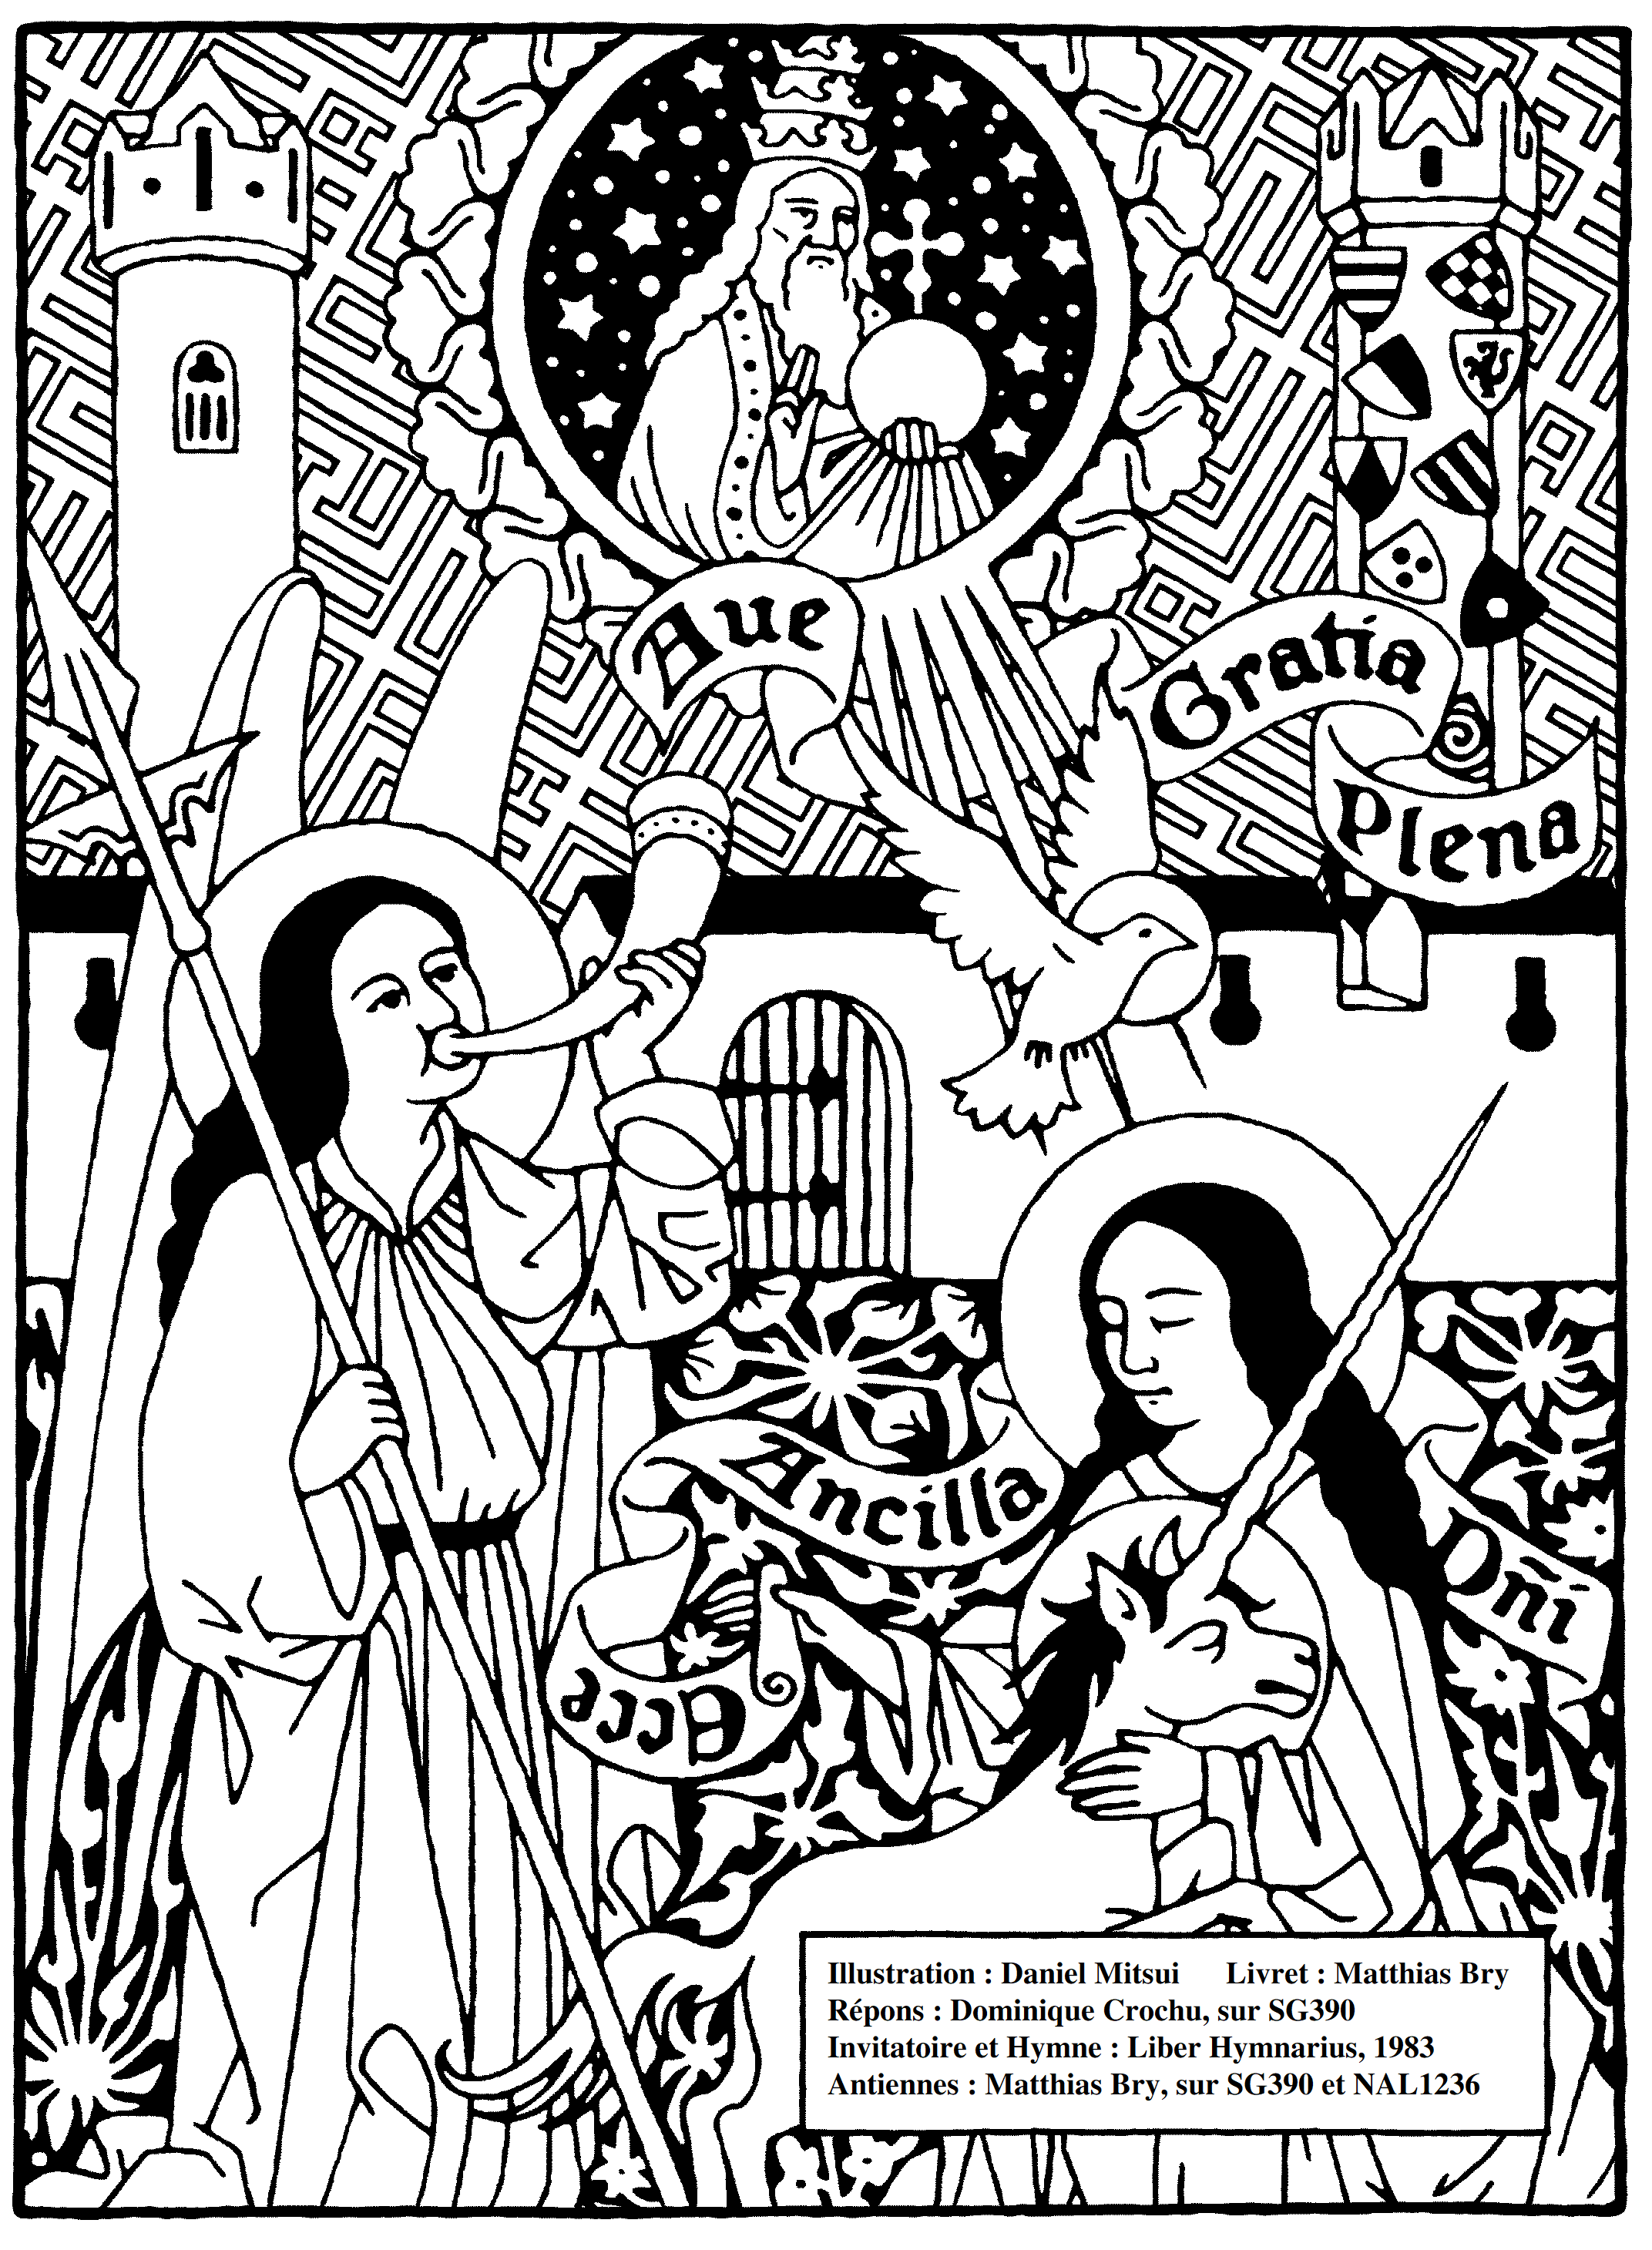
\includegraphics[width=13cm]{4ecouv.png}
\end{adjustwidth}
\end{document} 
